\subsection{Chat}

\begin{figure}[h!]
	\centering
	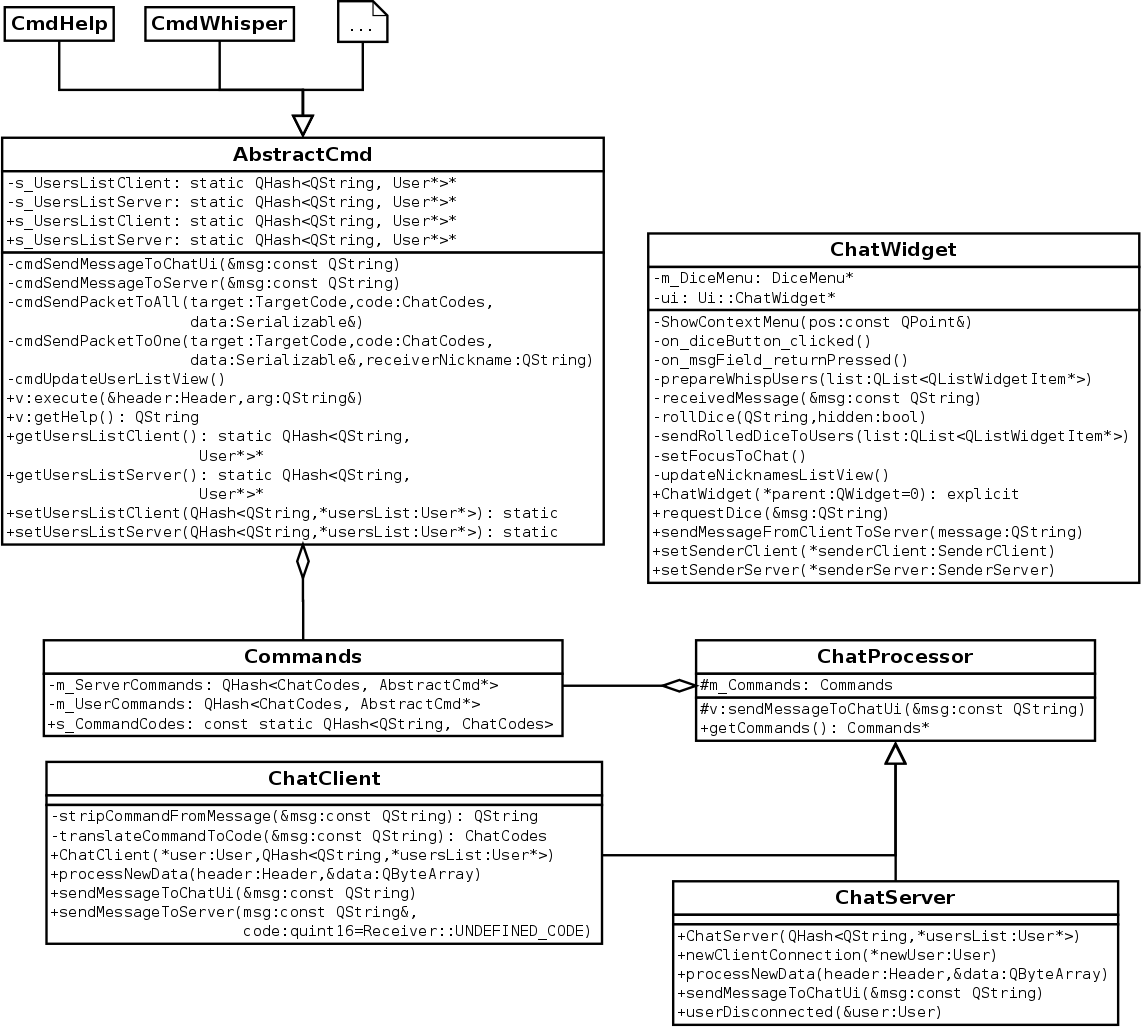
\includegraphics[width=\textwidth]{img/chat_uml.png}
	\caption{Diagramme UML du chat (seules quelques commandes ont été représentées pour éviter de surcharger le schéma)}
\end{figure}

Le Chat est constitué de la classe ChatWidget qui fait le lien entre l'interface graphique et les commandes qui peuvent être exécutées.\\

Lorsqu'une application est lancée, le pseudo souhaité par l'utilisateur est tout d'abord demandé. Ce pseudo n'est pas tout de suite utilisé, il est sauvegardé dans un attribut, et l'utilisateur est temporairement nommé \emph{guest}. La QTcpSocket se connecte ensuite au QTcpServer du MJ, et la méthode newClientConnection de ChatServer est appelée du côté du MJ. Cette méthode vérifie si le pseudo \emph{guest} est déjà pris et ajoute un tiret bas à la fin si c'est le cas (\emph{guest\_}), puis crée un User et l'ajoute à la liste des utilisateurs de SwitchServer et des modules réseau (ChatServer, MapServer, ...). Un message est ensuite envoyé au ChatClient de l'utilisateur venant de se connecter afin de le notifier de sa connexion et de son éventuel changement de pseudo si \emph{guest} était déjà utilisé. De plus, un message est envoyé à tous les autres clients afin de les prévenir de la connexion du nouvel utilisateur. Une fois ces étapes effectuées, l'utilisateur est connecté et est identifié par un pseudo unique. Enfin, le pseudonyme souhaité par l'utilisateur peut être utilisé : une demande de changement de pseudonyme est envoyée au ChatServer, des vérifications sont effectuées, puis le pseudonyme est validé et envoyé à tous les clients connectés. Ces étapes sont schématisées ci-dessous :

\begin{figure}[h!]
	\centering
	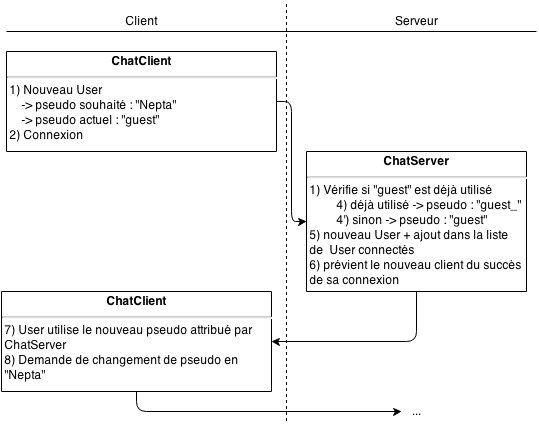
\includegraphics[width=0.7\textwidth]{img/chat_connection.png}
	\caption{Connexion \& identification d'un nouvel utilisateur}
\end{figure}

Cette identification pose plusieurs problèmes :
\begin{itemize}
	\item double affichage d'un message de changement de pseudonyme (guest, et pseudo souhaité);
	\item peu clair au niveau du code;
	\item l'identification est effectuée au niveau du chat, il serait cependant plus judicieux qu'un nouveau module ou que SwitchServer se charge de cette étape.
\end{itemize}

Une piste d'amélioration aurait été d'utiliser un module à part pour l'identification comme suggéré plus haut, ainsi que l'utilisation d'entiers pour identifier les joueurs plutôt que d'utiliser leurs pseudonymes.\\

Une fois connecté, l'utilisateur peut envoyer des messages et des commandes sur le chat via la zone de texte prévue à cet effet. Les commandes sont des classes héritant de AbstractCmd et doivent redéfinir les méthodes \emph{execute} et \emph{getHelp} qui correspondent respectivement à ce que va faire la commande et le message d'aide associé à celle-ci. Comme précisé précédemment, certaines commandes peuvent être lancées depuis le chat à l'aide d'une chaîne de caractères suivant le modèle suivant : \emph{/nom\_commande paramètres} \footnote{Ces commandes sont décrites dans la sous-section dédiée au chat dans la section manuel d'utilisation de ce rapport}. D'autres commandes sont exécutées en réponse à une autre commande, c'est par exemple le cas de la commande CmdNicknameAck qui est exécutée par un client en réponse à un paquet envoyé par le serveur lors d'un changement de pseudonyme (CmdNickname).\\

Toutes les commandes sont instanciées dans la classe Commands, qui elle même est instanciée par ChatClient et ChatServer, ainsi ces deux modules peuvent accéder aux commandes en utilisant la hashmap associant un code à une commande. Par exemple, le code \emph{ChatCodes::USERCMD\_HELP} est associé à la commande d'aide CmdHelp.\\